% $Header: /cvsroot/latex-beamer/latex-beamer/examples/beamerexample5.tex,v 1.22 2004/10/08 14:02:33 tantau Exp $

\documentclass[11pt]{beamer}

\usetheme{Darmstadt}

\usepackage{times}
\usefonttheme{structurebold}

%\usepackage[english]{babel}
\usepackage[portuges]{babel}
\usepackage{pgf,pgfarrows,pgfnodes,pgfautomata,pgfheaps}
\usepackage{amsmath,amssymb}
\usepackage[utf8]{inputenc}
\usepackage{graphicx}

\setbeamercovered{dynamic}

\newcommand{\Lang}[1]{\operatorname{\text{\textsc{#1}}}}

\newcommand{\Class}[1]{\operatorname{\mathchoice
  {\text{\sf \small #1}}
  {\text{\sf \small #1}}
  {\text{\sf #1}}
  {\text{\sf #1}}}}

\newcommand{\NumSAT}      {\text{\small\#SAT}}
\newcommand{\NumA}        {\#_{\!A}}

\newcommand{\barA}        {\,\bar{\!A}}

\newcommand{\Nat}{\mathbb{N}}
\newcommand{\Set}[1]{\{#1\}}

\pgfdeclaremask{tu}{beamer-tu-logo-mask}
\pgfdeclaremask{computer}{beamer-computer-mask}
\pgfdeclareimage[interpolate=true,mask=computer,height=2cm]{computerimage}{beamer-computer}
\pgfdeclareimage[interpolate=true,mask=computer,height=2cm]{computerworkingimage}{beamer-computerred}
\pgfdeclareimage[mask=tu,height=.5cm]{logo}{logounesp}

\logo{\pgfuseimage{logo}}
\title{Gases e Sólidos}
\author{Ney Lemke}
\institute[IBB-UNESP]{%
    Departamento de Biofísica e Farmacologia}
\date{\today}                                

\colorlet{redshaded}{red!25!bg}
\colorlet{shaded}{black!25!bg}
\colorlet{shadedshaded}{black!10!bg}
\colorlet{blackshaded}{black!40!bg}

\colorlet{darkred}{red!80!black}
\colorlet{darkblue}{blue!80!black}
\colorlet{darkgreen}{green!80!black}

\def\radius{0.96cm}
\def\innerradius{0.85cm}

\def\softness{0.4}
\definecolor{softred}{rgb}{1,\softness,\softness}
\definecolor{softgreen}{rgb}{\softness,1,\softness}
\definecolor{softblue}{rgb}{\softness,\softness,1}

\definecolor{softrg}{rgb}{1,1,\softness}
\definecolor{softrb}{rgb}{1,\softness,1}
\definecolor{softgb}{rgb}{\softness,1,1}

\AtBeginSection[]{\frame{\frametitle{Outline}\tableofcontents[current]}}

\begin{document}

\frame{\titlepage}

%\section*{Outline}

\part{Parte I}

\frame{\frametitle{Outline} 
\tableofcontents[part=1]}

\section{Introdução}
\frame{\frametitle{Mecânica Quântica}
  \begin{itemize}
  \item Níveis quantizados de energia evidências espectroscópicas
  \item Absorção e emissão ocorre apenas em frequências bem definidas
  \item $\Delta\epsilon=h\nu$
  \item Constante de Planck $h=6.626\times 10^{-34}J s$
  \end{itemize}

}
\frame{\frametitle{Exemplo}

  \begin{center}
    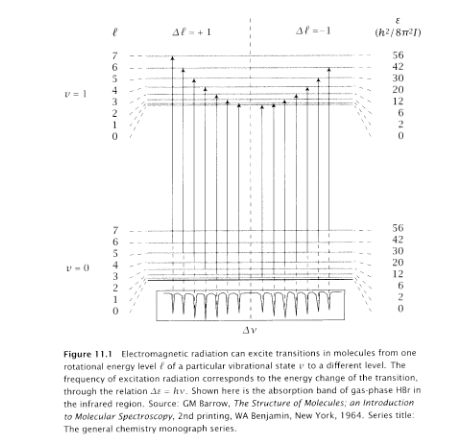
\includegraphics[scale=0.4]{niveisenergia}
  \end{center}
}

\frame{\frametitle{Espectro de Radiação}

 \begin{center}
    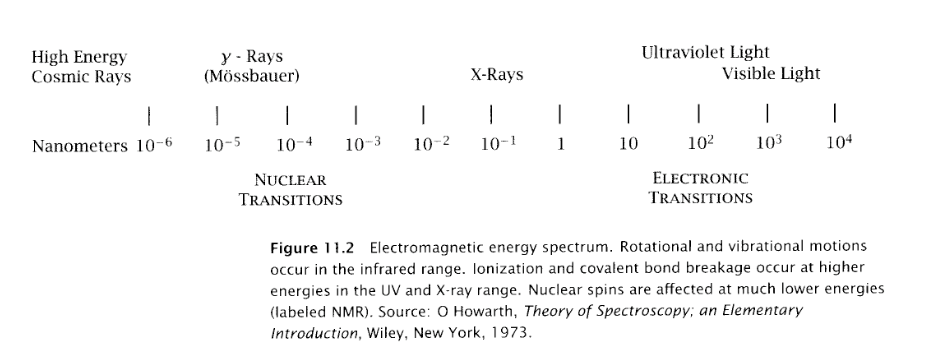
\includegraphics[scale=0.3]{espectro}
  \end{center}
}

\frame{\frametitle{Classes de Energia}
  \begin{itemize}
  \item Translacional
  \item Rotacional
  \item Vibracional
  \item Excitação Eletrônica
  \end{itemize}
}

\section{Mecânica Quântica}
\frame{\frametitle{Equação de Schrödinger}
$$H\psi=E_i\psi$$

$\psi=\psi(x,y,z)$ e $|\psi|^2$ representa a probabilidade
de encontrar a partícula em um ponto do espaço. 

$H$ é o hamiltoniano (ou hamiltoniana) do sistema. Ele representa a 
energia do sistema. Por exemplo para uma partícula sob a ação de um
potencial $V(x)$ temos:

$$H=\frac{p^2}{2m}+V(x)$$
}
\frame{\frametitle{Equação de Schrödinger}
  Na Mecânica Quântica $p^2$ é um operador  diferencial.

$$p^2=-\frac{h^2}{8\pi^2 m}\frac{\partial^2}{\partial x^2}$$
Neste caso:

$$H\psi =-\left( \frac{h^2}{8\pi^2 m}\right) \frac{\partial ^2\psi}{\partial x^2}
        +V(x)\psi=E_j\psi$$

onde $E_j$ são chamados de autovalores de energia. 
}

\frame{\frametitle{Poço de Potencial}

\begin{center}
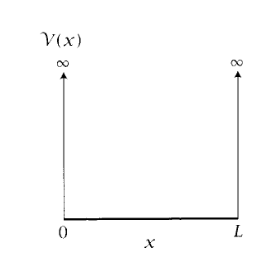
\includegraphics[scale=0.5]{poco}
\end{center}
}

\frame{\frametitle{Poço de Potencial}
$$\frac{d^2 \psi}{dx^2}+K^2\psi=0$$

$$K^2=\frac{8\pi^2 m \epsilon}{h^2}$$

$$\psi(x)=A \sin Kx + B \cos K x$$


}
\frame{\frametitle{Poço de Potencial}
Mas como $\psi(0)=\psi(L)$ $B=0$

$$\sin KL=0\quad KL=n\pi$$

$$\epsilon_n=\frac{(nh)^2}{8mL^2}$$

$$\psi_n (x)=\left(\frac{2}{L}\right)^{1/2} 
\sin\left( \frac{n\pi x}{L} \right)$$
}

\frame{\frametitle{Poço de Potencial}
\begin{center}
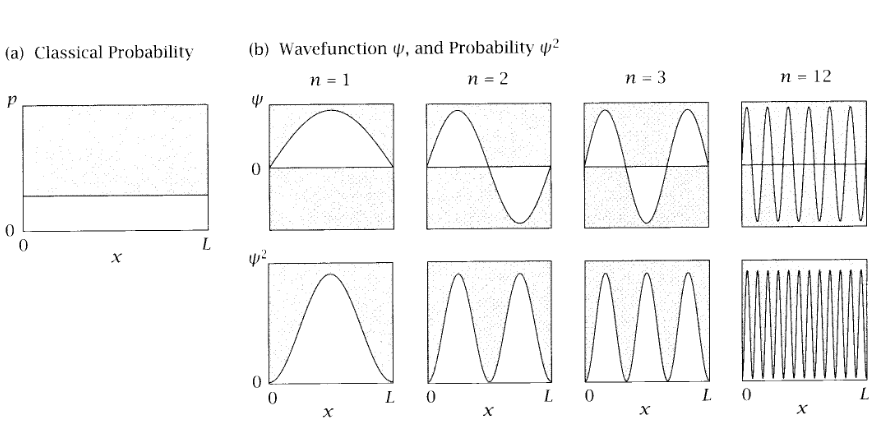
\includegraphics[scale=0.3]{psicaixa}
\end{center}

}


\frame{\frametitle{Exemplo}
Níveis de Energia para o argônio. $L=1$ cm $m=40$ g mol$^{-1}=0.040/6.02\times 10^{23} \mbox{atom mol}^{-1}$.

Neste caso temos que:

$$\epsilon=n^2\frac{(6.626\times10^{-34}\mbox{Js})^2}{8 6.64\times 10^{-26}\mbox{kg} (10^ {-2} \mbox{m})^2}=n^2(8.27\times10^{-39}) \mbox{J}$$


}
\section{Translação}

\frame{\frametitle{Função Partição de Translação}

$$q_{trans}=\sum_{n=1}^\infty e^{-\epsilon_n/KT}=
           \sum_{n=1}^\infty e^{-n^2h^2/8mL^2kT}
$$

$$\theta_{trans}=\frac{h^2}{8 m L^2}$$

$$q_{trans}=\sum_{n=1}^\infty  e^{-n^2\theta/T}
$$
}
\frame{\frametitle{Função Partição de Translação}
Se $\theta<<1$, o que é geralmente o caso para temperaturas 
proximas a temperatura ambiente. Podemos aproximar 
o somatório por uma integral. 
$$q_{trans}=\int_0^\infty e^{-(h^2/8mL^2 k T)n^2}dn=
\left(\frac{2 \pi m kT}{h^2} \right)^{1/2}L$$
}


\frame{\frametitle{Partícula em uma Caixa 3D}
$$-\frac{h^2}{8\pi^2m}\left( \frac{\partial^2}{\partial x^2}+
                          \frac{\partial^2}{\partial y^2}+
                          \frac{\partial^2}{\partial z^2}\right)
\psi+{\cal V}(x,y,z)\psi=\epsilon\psi
$$

$${\cal V}(x,y,z)=0$$ apenas no interior de uma caixa de lados $a$, $b$ e $c$
e infinito em todos pontos.
}

\frame{\frametitle{Partícula em uma Caixa 3D}
$$H_x\psi_x=\epsilon_x$$
$$H_y\psi_y=\epsilon_y$$
$$H_z\psi_z=\epsilon_z$$

Neste caso:

$$H_x=-\frac{h^2}{8\pi^2 m}\left(\frac{\partial^2}{\partial x^2}\right)$$

$$\psi(x,y,z)=\psi_x(x)\psi_y(y)\psi_z(z)$$

$$\epsilon_{n_x,n_y,n_z}=\frac{h^2}{8 m}\left(  \frac{n_x^2}{a^2}+ 
                                                \frac{n_y^2}{b^2}+
                                                \frac{n_z^2}{c^2}
                                              \right)$$

}
\frame{\frametitle{Partícula em uma Caixa 3D}

  $$q_{trans}=q_xq_yq_z=\left(\frac{2 \pi m kT}{h^2} \right)^{3/2}V
            =\frac{V}{\Lambda^3}$$

$$\Lambda^3=\left(\frac{h^2}{2 \pi m k T} \right)^{3/2}$$

Ex. $\Lambda=0.714 \AA$ para H$_2$ em $T=300 K$. 

Ex. Argônio em $T=273 K$ 

$V=2.24\times 10^{-2}$m$^3$ $q_{trans}=2.14\times10^{30}$
}


\frame{\frametitle{Energia}
$$H=H_{trans}+H_{vib}+H_{rot}+H_{elet}$$


$$\psi=\psi_{trans}\psi_{vib}\psi_{rot}\psi_{elet}$$
}



\section{Vibração}

\frame{\frametitle{Oscilador Harmônico}

$$-\frac{h^2}{8\pi^2m}\frac{d^2\psi (x)}{dx^ 2}+\frac{1}{2}k_sx^ 2\psi(x)=\epsilon_v\psi(x)$$

$$\epsilon_v=h\nu(v+\frac{1}{2})$$

$\nu=(1/2\pi)(k_s/m)^{(1/2)}$ e $v=0,1,2,\ldots$

\begin{center}
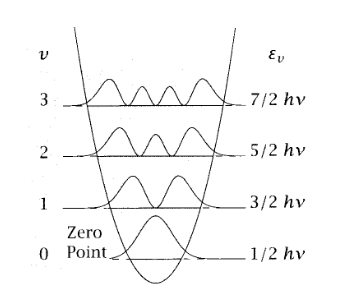
\includegraphics[scale=0.3]{oscilador}  
\end{center}
}

\frame{\frametitle{Molécula diatômica}
\begin{center}
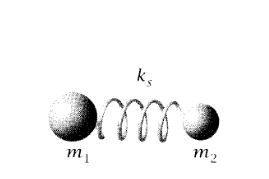
\includegraphics[scale=0.3]{duasmassas}  
\end{center}

$$\epsilon_v=h\nu(v+\frac{1}{2})$$

$$\nu=(1/2\pi)(k_s/\mu)^{(1/2)}$$
$$v=0,1,2,\ldots$$
$$\mu=\frac{m_1m_2}{m_1+m_2}$$


}


\frame{\frametitle{Molécula diatômica}
A função partição neste caso é:


$$q_{vib}=\sum_{v=0}^\infty e^{-(v+1/2)h\nu/kT}=e^{-h\nu/2kT}(1+e^{-hv/kT}+
                                                    e^{-2hv/kT}\ldots)$$
$$q_{vib}=\frac{e^{-h\nu/2kT}}{1-e^{-h\nu/kT}}$$

}

\section{Rotação}

\frame{\frametitle{Rotor Clássico}

\begin{center}
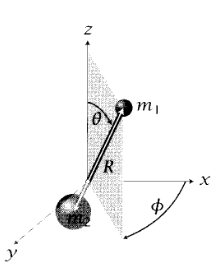
\includegraphics[scale=0.3]{rotor}  
\end{center}
}
\frame{\frametitle{Força Central}
$$H=\frac{p_1^2}{2 m_1}+\frac{p_2^2}{2 m_2}+V(|\vec{r_1}-\vec{r_2}|)$$
 \begin{tabular}{c c}
    \begin{minipage}{0.45\textwidth}

%\includegraphics[scale=0.5]{forcacentral}

    \end{minipage}&
    \begin{minipage}{0.45\textwidth}
$$\vec{p_1}=m_1\vec{v_1} \quad \vec{p_2}=m_2 \vec{v_2}$$

$$M=m_1+m_2$$


    \end{minipage}
  \end{tabular}
} 

\frame{\frametitle{Coordenadas reduzidas}

$$\vec{r}=\vec{r_2}-\vec{r_1} \quad \vec{r_G}=\frac{m_1 \vec{r_1} +m_2\vec{r_2}}{M}$$

$$\vec{r_1}=\vec{r_G}+\frac{m_2 \vec{r}}{M} \quad 
\vec{r_2}=\vec{r_G}-\frac{m_1 \vec{r}}{M}$$

$$H=\frac{1}{2}M\dot{\vec{r_G}^2}+\frac{1}{2M}\dot{\vec{r}}^2m_1m_2+V(r)$$ 

$$H=\frac{\dot{\vec{p_G}^2}}{2M}+\frac{\dot{\vec{p}}^2}{2\mu}+V(r)$$

$$\mu=\frac{m_1m_2}{m_1+m_2}$$


}

\frame{\frametitle{Momento Angular Clássico}
Em coordenadas esféricas temos:

$$\vec{L}=\mu \vec{v}\times \vec{r}$$

$$=\mu (\dot{\vec{r}}\vec{a_r}+r\dot{\theta}\vec{a_\theta}+r\sin \theta \dot{\phi}\vec{a_\phi})\times \vec{r}$$

$$=\mu (r^2\dot{\theta}^2\vec{a_\phi}+r^2\sin \theta \dot{\phi}\vec{a_\theta})$$

$$L^2=\mu^2r^4(\dot{\theta}^2+\sin^2 \theta\dot{\phi ^2})$$

}
\frame{\frametitle{Momento Angular Clássico}

$$\frac{\mu v^2}{2}=\frac{\mu}{2}(\dot{r}^2+r^2\dot{\theta}^2+r^2\sin^2 \theta \dot{\phi}^2)$$

$$\frac{\mu v^2}{2}=\frac{p^2}{2\mu }=\frac{\mu}{2}\dot{r}^2+\frac{L^2}{2\mu r^2}$$

Neste caso temos que $\dot{r}=0$, e $r=R$. 

$$\frac{p^2}{2\mu}=\frac{L^2}{2\mu R^2}$$
}



\frame{\frametitle{Rotor Quântico}

$$H\psi_{\cal l}=\frac{L^2\psi}{2\mu R^2}=\epsilon\psi_{\cal l}$$

$$\epsilon_l=\frac{{\cal l}({\cal l}+1)h^2}{8\pi^2I}$$

$l=0,1,2,\ldots$

$$q_{rot}=\sum_{l=0}^\infty (2l+1)e^{-\epsilon_l/kT}$$
}

\frame{\frametitle{Rotação}
Para altas temperaturas temos que:

$$q_{rot}=8\frac{\pi^2IkT}{\sigma h^2}$$

onde  $\sigma$ depende do número de orientações equivalentes das
moléculas.

\begin{description}
\item[$\sigma=1$ ] moléculas diatômicas heteronucleares
\item[$\sigma=2$] moléculas diatômicas homonucleares
\item[$\sigma=12$] benzeno
\end{description}
}


\section{Níveis Eletrônicos}

\frame{\frametitle{Níveis Eletrônicos} Estes termos são mais difíceis
  de determinar pois dependem de rearranjos eletrônicos. Não vamos
  entrar em detalhes para estes fatores.
}

\frame{\frametitle{Função Partição}

$$q=\left[\frac{2 \pi m kT}{h^2} \right]^{3/2}V\left[ \frac{\pi^2IkT}{\sigma h^2}\right]\left[\frac{e^{-h\nu/2kT}}{1-e^{-h\nu/kT}}\right]$$
}


\section{Gases Ideais}

\frame{\frametitle{Pressão}


$$q=q_1V$$

$$Q=\frac{q^N}{N!}$$

Usando Stirling temos que: 

$$F=-kT\ln Q=-kTN\ln \frac{eq}{N}$$

$$p=-\left( \frac{\partial F}{\partial V} \right)_{T,N}=\frac{NkT}{V}$$
}

\frame{\frametitle{Energia Interna}

$$U=NkT^2\left( \frac{\partial \ln q}{\partial T}\right)$$

$$U=\frac{3}{2}NkT+NkT$$

Além destes termos temos ainda os termos provenientes das vibrações.
}

\frame{\frametitle{Entropia}

  Consideramos neste caso gases formados por moléculas monoatômicas.

$$S=k\ln\left( \frac{q^N}{N!}\right)+\frac{U}{T}=Nk\ln q-k(N\ln N -N)
   +\frac{3}{2}Nk$$

$$S=Nk\ln \left( \frac{qe^{5/2}}{N} \right)$$

$$S=Nk\left[\left( \frac{2 \pi m kT}{h^2}\right) \left(\frac{e^{5/2}}{N}\right) V
\right]  $$

  }
\section{Equipartição de Energia}


\frame{\frametitle{Equipartição de Energia}

Observamos anteriormente que cada grau de liberdade recebe 
a mesma quantidade de energia $kT/2$. Como podemos demonstrar este resultado?



$$\langle \epsilon \rangle =\frac{\sum \epsilon(x)e^ {-\epsilon(x)/kT}}{\sum e^ {-\epsilon(x)/kT}}$$

No caso dos efeitos quânticos serem desprezíveis

$$\langle \epsilon \rangle =\frac{\int_{-\infty}^\infty \epsilon(x)e^ {-\epsilon(x)/kT}dx}
{\int_{-\infty}^\infty e^ {-\epsilon(x)/kT}dx}$$
}


\frame{\frametitle{Equipartição de Energia}
Em muitos casos de interesses $\epsilon=cx^2$ neste caso:

$$\langle \epsilon \rangle =\frac{\int_{-\infty}^\infty cx^2e^ {-\epsilon(x)/kT}dx}
{\int_{-\infty}^\infty e^ {-\epsilon(x)/kT}dx}=\frac{1}{2}kT$$

No caso de um gás monoatômico temos que:
$$C_v=\left( \frac{\partial U}{\partial T}\right) =\frac{3}{2}Nk$$

Ou seja o calor específico molar é $C_v=3R/2$ para gases monoatômicos.
}

\frame{\frametitle{Modelo de Einstein}
Este argumento não é válido para modos vibracionais. Neste caso
podemos mostrar que:

$$q=(1-e^{-\beta h \nu})^{-1}$$

$$\langle \epsilon \rangle =-\frac{1}{q}\left( \frac{\partial q}{\partial \beta}
\right)=h\nu\left( \frac{e^{-\beta h \nu}}{1-e^{-\beta h \nu}}\right)$$

$$C_v=3N\left( \frac{\partial \langle\epsilon\rangle}{\partial T}
\right)=3Nk\left(\frac{h\nu}{kT}\right)^2\frac{e^{-h \nu/kT}}{(1-e^{-h\nu /kT})^2}
$$
}
\frame{\frametitle{Modelo de Einstein}
  \begin{center}
    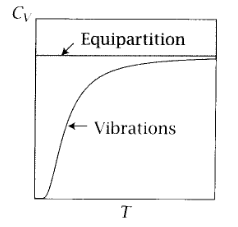
\includegraphics[scale=0.5]{einstein1}
  \end{center}

}



\frame{\frametitle{Modelo de Einstein}
  \begin{center}
    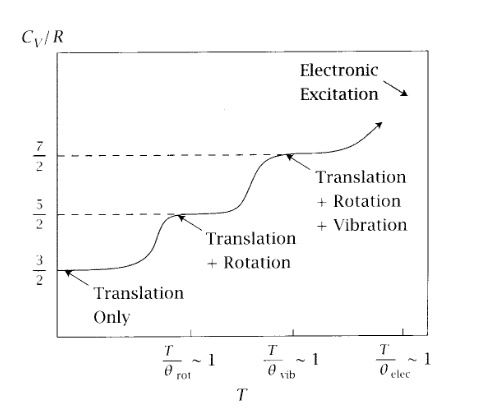
\includegraphics[scale=0.5]{einstein2}
  \end{center}

}

\frame{\frametitle{Modelo de Einstein}
  \begin{center}
    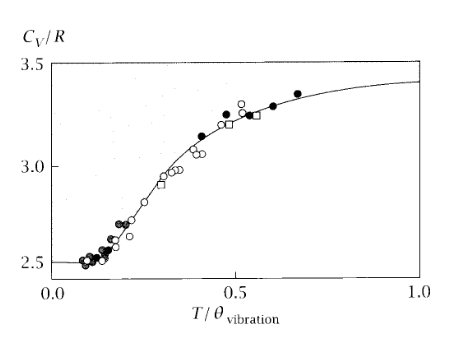
\includegraphics[scale=0.5]{einstein3}
  \end{center}

}

\frame{\frametitle{Modelo de Einstein}
  \begin{center}
    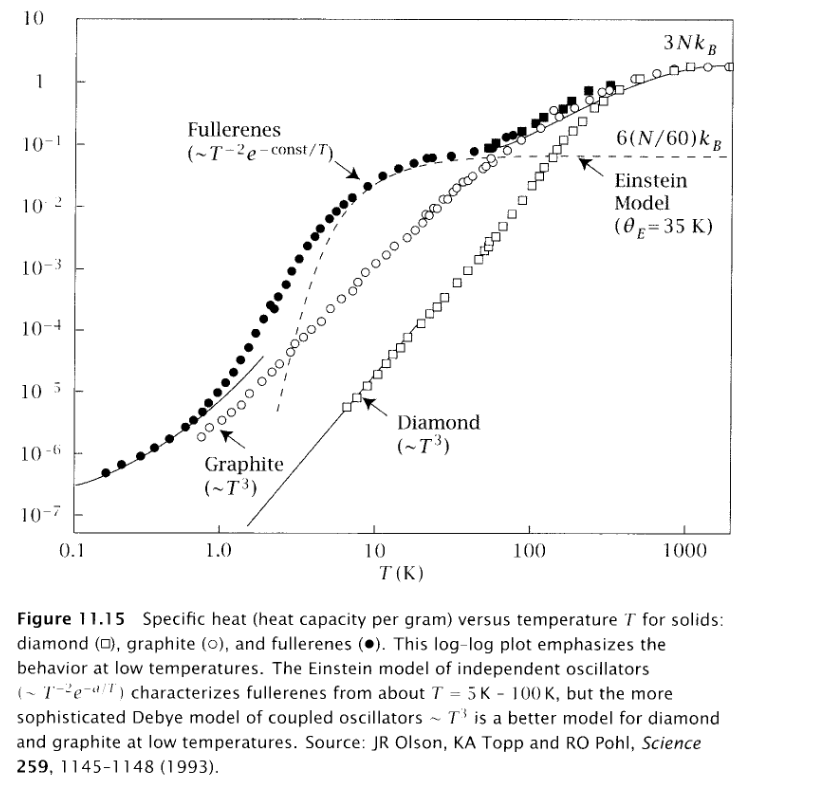
\includegraphics[scale=0.2]{einstein4}
  \end{center}

}
\end{document}
